\documentclass[conference]{IEEEtran}
\IEEEoverridecommandlockouts
\usepackage{cite}
\usepackage{amsmath,amssymb,amsfonts}
\usepackage{algorithmic}
\usepackage{graphicx}
\usepackage{textcomp}
\usepackage{xcolor}
\usepackage[utf8]{inputenc}
\usepackage{booktabs}
\usepackage{multirow}
\usepackage{array}

\def\BibTeX{{\rm B\kern-.05em{\sc i\kern-.025em b}\kern-.08em
    T\kern-.1667em\lower.7ex\hbox{E}\kern-.125emX}}

\begin{document}

\title{Adaptive Retrieval-Augmented Generation Framework with Hybrid Retrieval and Intent-Aware Context Optimization}

\author{%
\IEEEauthorblockN{\textbf{G. Sai Preetham}}
\IEEEauthorblockA{\textit{Dept.~of Computational} \\ \textit{Intelligence}\\%
SRM Institute of Science and \\ Technology\\%
Kattankulathur, India\\%
sg9499@srmist.edu.in}
\and
\IEEEauthorblockN{\textbf{Dr. Sasi Rekha Sankar}}
\IEEEauthorblockA{\textit{Dept.~of Computational} \\ \textit{Intelligence}\\%
Faculty of Engineering and \\Technology\\%
SRM Institute of Science and \\ Technology\\%
Kattankulathur, India\\%
sasireks@srmist.edu.in}
\and
\IEEEauthorblockN{\textbf{Karan Dhillon}}
\IEEEauthorblockA{\textit{Dept.~of Computational} \\ \textit{Intelligence}\\%
SRM Institute of Science and \\ Technology\\%
Kattankulathur, India\\%
kd2803@srmist.edu.in}
}

\maketitle

%----------------------------------------------------------------
\begin{abstract}
Retrieval-Augmented Generation (RAG) augments large language
models (LLMs) with external knowledge retrieved at inference
time, yet standard pipelines suffer from two compounding
failure modes: \emph{context bloat}, wherein naively
concatenating retrieved chunks wastes tokens on low-relevance
content, and \emph{uniform retrieval}, wherein dense vector
search ignores lexical overlap and query intent. We present
an \emph{Adaptive RAG} system that resolves both limitations
through a four-stage pipeline: (i)~hybrid dense--sparse
retrieval combining FAISS~\cite{johnson2021billion} with
BM25~\cite{robertson1995okapi} via min-max normalized score
fusion, (ii)~diversity-aware shortlisting enforcing
per-section caps prior to reranking, (iii)~cross-encoder
reranking~\cite{nogueira2019passage} augmented by
query-intent-conditional scoring, and (iv)~a dual-stage
compression module combining sentence-level intent scoring
with a 0/1 knapsack optimizer under a hard token budget. A
protected-chunk mechanism ensures the top-3 highest-scoring
passages appear verbatim. Controlled evaluation demonstrates
approximately 33.33\% average token reduction (up to 57.94\%) while preserving
answer-bearing content.

\smallskip\noindent\textbf{Key contributions:}
\begin{itemize}
  \item Hybrid dense--sparse retrieval with min-max normalized
        score fusion and diversity-aware shortlisting prior to
        cross-encoder reranking.
  \item A five-category rule-based intent detection mechanism
        conditioning both retrieval scoring (up to $+0.30$)
        and sentence-level evidence prioritization.
  \item A dual-stage compression module: intent-aware sentence
        scoring followed by 0-1 knapsack selection under a
        hard budget, with a top-3 protected-chunk guarantee.
  \item An A/B evaluation framework enabling direct
        token-efficiency comparison across intent categories.
\end{itemize}
\end{abstract}

\begin{IEEEkeywords}
Retrieval-Augmented Generation, hybrid retrieval, BM25, FAISS,
cross-encoder reranking, context compression, query intent
detection, knapsack optimization, large language models
\end{IEEEkeywords}

%----------------------------------------------------------------
\section{Introduction}

Retrieval-Augmented Generation (RAG) \cite{lewis2020rag}
grounds LLM outputs in non-parametric external knowledge by
conditioning generation on retrieved text, mitigating the
inability of parametric models to access up-to-date or
domain-specific facts without retraining. Practical RAG
deployments over long technical documents face two critical
challenges.

\textit{Context bloat.} LLMs have finite context windows;
concatenating the top-$k$ retrieved chunks reduces the
signal-to-noise ratio and, in extreme cases, causes the model
to overlook the correct answer \cite{beltagy2020longformer,
lewis2020rag}. While modern language models support large
context windows, processing excessive context increases
latency, raises computational cost, and diminishes attention
to relevant information---commonly termed the
``lost in the middle'' effect \cite{beltagy2020longformer}.
Efficient context selection therefore remains critical for
practical RAG systems.

\textit{Uniform retrieval.} Dense vector similarity treats
all queries identically, ignoring lexical overlap and query
semantics. A query asking ``What accuracy was achieved?''
requires numerically dense result-section evidence, whereas
``How does the algorithm work?'' demands methodological
exposition. A single cosine-similarity ranking cannot
distinguish these needs \cite{karpukhin2020dpr}.

Prior work addresses each challenge in isolation.
Efficient transformers (Longformer \cite{beltagy2020longformer},
BigBird \cite{zaheer2020bigbird}) scale input length but still
ingest irrelevant tokens. ColBERT \cite{khattab2020colbert}
improves precision without compressing the generator's context.
Extractive summarizers (TextRank \cite{mihalcea2004textrank},
LexRank \cite{erkan2004lexrank}) are query-agnostic.
Abstractive compressors (BART \cite{lewis2020bart}, PEGASUS
\cite{zhang2020pegasus}) risk hallucinating away critical
numerical or API details. FiD \cite{izacard2021fid} context
grows linearly with retrieved passages, making token-budget
enforcement intractable.

The guiding principle of this work is to \emph{retrieve broadly, yet supply only a narrow, intent-focused context to the generator.} The Adaptive RAG
pipeline (i)~retrieves a large candidate pool via hybrid
dense--sparse retrieval, (ii)~applies intent-conditioned
diversity-aware shortlisting, (iii)~reranks with an
intent-augmented cross-encoder, and (iv)~compresses the context
at sentence granularity via \emph{intent-aware evidence
prioritization} and a \emph{0/1 knapsack optimizer} enforcing
a hard token budget---with the top-3 highest-scoring passages
always protected. The result is a quantifiably compact,
evidence-focused context that supports accurate long-document
QA under strict token constraints.

%----------------------------------------------------------------
\section{Related Work}

\textbf{Long-Context Transformers.}
Longformer \cite{beltagy2020longformer} and BigBird
\cite{zaheer2020bigbird} reduce the $O(n^2)$ attention cost
via sparse patterns, enabling thousands of input tokens.
However, they scale \emph{input length} rather than performing
evidence selection: irrelevant tokens are still processed,
wasting compute.

\textbf{Dense and Sparse Retrieval.}
DPR \cite{karpukhin2020dpr} retrieves passages by semantic
vector similarity. ColBERT \cite{khattab2020colbert} preserves
contextualized token embeddings for late-interaction reranking.
Both operate at passage level without intra-passage compression
or token-budget enforcement. BM25 \cite{robertson1995okapi}
anchors on exact lexical overlap, complementing semantic search.

\textbf{Retrieval-Augmented Generation.}
Lewis et al.\ \cite{lewis2020rag} combine DPR with a
sequence-to-sequence generator. FiD \cite{izacard2021fid}
encodes passages independently before decoder fusion. Both
retrieve entire passages without fine-grained compression.

\textbf{Context Compression.}
TextRank \cite{mihalcea2004textrank} and LexRank
\cite{erkan2004lexrank} rank sentences by global document
importance, not query relevance. SummaRuNNer
\cite{nallapati2017summarunner} is supervised but lacks
token-budget enforcement. Abstractive methods (T5
\cite{raffel2020t5}, BART \cite{lewis2020bart}, PEGASUS
\cite{zhang2020pegasus}) risk paraphrasing away exact
numerical or API details. Our approach is extractive,
query-aware, and model-agnostic.

Recent work on prompt compression, such as LLMLingua and Selective Context, focuses on token-level pruning or heuristic filtering. However, these approaches operate independently of retrieval ranking and do not incorporate query-aware optimization under a fixed budget constraint.

\textbf{Hallucination and Faithfulness.}
SelfCheckGPT \cite{manakul2023selfcheckgpt} detects
hallucinations post-generation. TruthfulQA
\cite{lin2022truthfulqa} benchmarks factual reliability.
Neither work proactively removes low-signal context.

\textbf{Scientific Document Structure.}
Lo et al.\ \cite{lo2020s2orc} demonstrate that naive chunking
breaks semantic coherence across structured academic sections,
motivating our section-aware diversity filtering.

%----------------------------------------------------------------
\section{Proposed Methodology}

\begin{figure}[htbp]
    \centering
    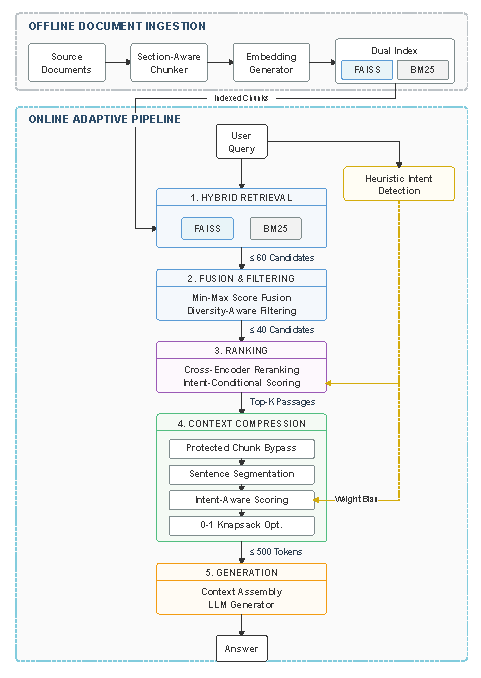
\includegraphics[width=\columnwidth]{architecture_diagram.pdf}
    \caption{System architecture of the Adaptive RAG pipeline. The framework utilizes a dual-index hybrid retrieval mechanism, routing queries through a heuristic intent detector. The core contribution, the Context Compression Module, optimizes token utilization via 0-1 Knapsack segmentation, progressively funnelling candidate passages into a high-density prompt.}
    \label{fig:pipeline}
\end{figure}

Figure~\ref{fig:pipeline} illustrates the complete pipeline.

\subsection{Query Intent Detection}
The system classifies each user query into one of five semantic
intent categories: \textsc{Result}, \textsc{Method}, \textsc{Api\_Usage}, \textsc{Definition},
and \textsc{Comparison}. For each category $k$, a weighted phrase-match
score is computed over a curated keyword-phrase set $\mathcal{K}_k$
(e.g., ``accuracy'', ``how does'', ``is defined as''):
%
\begin{equation}
r_k = \frac{\displaystyle
  \sum_{p \in \mathcal{K}_k} |p|_w \cdot
  \mathbf{1}[p \sqsubseteq q_{\downarrow}]}
  {|\mathcal{K}_k|}
\label{eq:rawscore}
\end{equation}
%
where $|p|_w$ is the word count of phrase $p$, and
$p \sqsubseteq q_{\downarrow}$ denotes a substring match in
the lowercased query. Multi-word phrases (e.g., ``how does'',
weight~2) are rewarded over single-word keywords. Confidence
is then scaled and boosted for multi-keyword queries:
%
\begin{equation}
c_k = \min\!\left(2\,r_k +
  0.2 \cdot \mathbf{1}\!\left[m_k \geq 2\right],\;1.0\right)
\label{eq:confidence}
\end{equation}
%
where $m_k$ counts distinct matched phrases. The winning
intent $k^* = \arg\max_k c_k$ is applied if
$c_{k^*} > \tau_c = 0.30$; otherwise the system falls back
to DEFINITION. The rule-based formulation enables deterministic behavior, interpretability, and negligible latency overhead, making it suitable for real-time deployment scenarios.

\subsection{Hybrid Dense--Sparse Retrieval}
An initial candidate pool of size
$K = \min\!\left(\max\!\left(4\,\mathrm{top}_k,\,12\right),60\right)$
is retrieved from two independent indexes:
\begin{itemize}
  \item \textbf{Dense}: Exact inner-product search over
        L2-normalized \texttt{BAAI/bge-large-en} embeddings
        (1024-dimensional); the inner product on unit vectors corresponds to cosine similarity.
  \item \textbf{Sparse}: Okapi BM25 \cite{robertson1995okapi}
        over whitespace-tokenized chunk texts, capturing exact lexical overlap.
\end{itemize}

Both score lists are independently min-max normalized to
$[0,1]$, then fused:
%
\begin{equation}
s_{\mathrm{hybrid}}^{(i)} =
  0.5\,\tilde{s}_{\mathrm{dense}}^{(i)} +
  0.5\,\tilde{s}_{\mathrm{sparse}}^{(i)}
\label{eq:hybrid}
\end{equation}
%
Score normalization provides a simple mechanism for combining heterogeneous retrieval signals. Chunks present in only one index receive $0$ on the absent
dimension, preserving single-retriever candidates with partial
credit. A \textbf{diversity-aware shortlisting} step then
enforces a per-section cap before reranking:
%
\begin{equation}
\mathrm{cap}_{\mathrm{sec}} =
  \max\!\left(2,\left\lfloor\frac{N_{\max}}{\mathrm{top}_k}
  \right\rfloor\right),\quad N_{\max}=40
\label{eq:cap}
\end{equation}
%
At most $\mathrm{cap}_{\mathrm{sec}}$ chunks from any single
document section advance to reranking, preventing thematic
domination common in structured academic documents
\cite{lo2020s2orc}.

\subsection{Cross-Encoder Reranking with Intent-Conditional Scoring}
A cross-encoder reranking model (e.g., \texttt{ms-marco-MiniLM-L-6-v2})
\cite{nogueira2019passage} jointly scores up to 40
$(q,\,p_i)$ candidate pairs, producing fine-grained relevance
scores $s_{\mathrm{rerank}}^{(i)}$. To incorporate query semantics, the final composite score
is formulated as:
%
\begin{equation}
s_{\mathrm{final}}^{(i)} = 0.6\,s_{\mathrm{rerank}}^{(i)}
  + 0.3\,\tilde{s}_{\mathrm{dense}}^{(i)}
  + 0.1\,\tilde{s}_{\mathrm{sparse}}^{(i)}
  + b_{\mathrm{intent}}^{(i)}
\label{eq:finalscore2}
\end{equation}
%
The intent bonus $b_{\mathrm{intent}}^{(i)} \leq 0.30$
rewards chunks structurally aligned with the detected intent.
Exemplary rules include:
\textsc{Result} queries receive $+0.15$ for result-section membership,
$+0.10$ for digit-containing text, and $+0.05$ for percentage
symbols; \textsc{Api\_Usage} queries receive up to $+0.20$ for
a high density of code symbols; \textsc{Definition} queries receive $+0.20$ for
abstract or introduction section membership. All bonuses are
applied only when the intent confidence $c_{k^*} > 0.30$. Table~\ref{tab:scoring}
provides the complete scoring reference. All scoring weights and threshold values were empirically determined through grid search on a held-out validation subset of queries to ensure stable performance across different query types.

\subsection{Dual-Stage Context Compression}

\subsubsection{Protected-Chunk Inclusion}
The top-3 chunks by $s_{\mathrm{final}}$ are designated
\emph{protected} and included verbatim in the output context
(labeled \texttt{[PROTECTED]}). Their estimated token cost
$T_p = \lfloor|C_p|/4\rfloor$ is subtracted from the global
budget $T_{\max}$, leaving:
$T_r = \max(T_{\max} - T_p,\,0)$
for evidence selection over the remaining chunks. In cases where the protected chunks alone exceed the predefined token budget, truncation is applied in descending order of relevance to maintain adherence to the constraint.

\subsubsection{Intent-Aware Sentence Scoring}
Sentences are extracted from non-protected chunks using a
rule-based boundary detection heuristic relying on punctuation and capitalization.
Each sentence $s_j$ is scored by four generic factual signals
and an intent-specific component to quantify its standalone value:
%
\begin{align}
\mathrm{score}(s_j) &=
  0.06\,\delta_{\mathrm{digit}} +
  0.04\,\delta_{\mathrm{acronym}} \notag \\
&\quad +\,0.03\,\delta_{\mathrm{compound}} +
  0.03\,\delta_{\mathrm{alphanum}} \notag \\
&\quad +\,f_{\mathrm{intent}}(s_j, k^*)
\label{eq:sentence}
\end{align}
%
where the four binary indicator functions $\delta_{\cdot}$
detect: a digit ($\delta_{\mathrm{digit}}$), an uppercase
acronym of $\geq$2 consecutive capitals
($\delta_{\mathrm{acronym}}$), a hyphenated or slashed identifier
such as \textit{top-1} ($\delta_{\mathrm{compound}}$), and a
letter-prefixed numeric token such as \textit{bge-large}
($\delta_{\mathrm{alphanum}}$).
When the intent confidence is low ($c_{k^*} \leq 0.30$), $f_{\mathrm{intent}} = 0$, and the sentence scoring gracefully degrades to a length-based heuristic, prioritizing longer informative sentences.
Table~\ref{tab:scoring} lists the intent-specific bonuses
for $f_{\mathrm{intent}}$.

\subsubsection{0-1 Knapsack Optimization}
To maximize the informational value of the context under a strict token ceiling, the optimal sentence subset is found by solving the 0-1 knapsack problem:
%
\begin{equation}
\max\sum_j v_j x_j \quad
\text{s.t.}\;\sum_j w_j x_j \leq T_r,\;
x_j \in \{0,1\}
\label{eq:knapsack}
\end{equation}
%
where $v_j = \mathrm{score}(s_j)$ and
$w_j = \lfloor|s_j|/4\rfloor$ (token count estimate). Token estimation using character-length approximation serves as a lightweight proxy suitable for real-time optimization constraints.
The dynamic programming (DP) recurrence over a pool capped at 40 sentences is:
%
\begin{equation}
dp[i][w] = \max\!\left(dp[i{-}1][w],\;
  dp[i{-}1][w{-}w_i] + v_i\right), \quad w_i \leq w
\label{eq:dp}
\end{equation}
%
The time complexity of the DP algorithm is $O(40 \cdot T_r)$, rendering it highly tractable for typical token budgets. Sentences are selected based on their relevance scores and inserted in descending order of importance; a subsequent greedy pass
enforces the hard token ceiling.

\subsection{Answer Generation}
The final compressed context, formed by concatenating the protected passages and the knapsack-selected sentences
($C_{\mathrm{final}} = C_{\mathrm{protected}} \,\|\, C_{\mathrm{compressed}}$),
is passed to the LLM alongside the user query:
\begin{quote}
\small\textit{You are a technical QA system.
Context: \{context\}.
Question: \{query\}.
Answer clearly and concisely.}
\end{quote}
The system is designed to be model-agnostic, supporting multiple large language model backends (e.g., LLaMA 3.3 and Gemini) to ensure robustness and deployment flexibility.


%----------------------------------------------------------------
\section{System Architecture and Implementation}

\subsection{Document Ingestion and Indexing}
Source documents are systematically parsed into raw text. A regex-based section detector scans the
first ten lines of each page for structural headers shorter than
50 characters (e.g., ``Abstract'', ``Methodology'',
``Results''), propagating the semantic label forward to subsequent unlabeled
pages. Text is then segmented using a sentence-boundary
heuristic. To construct passages, sentences are greedily accumulated
until adding the next would exceed an 850-character limit; a new
chunk then begins with the trailing 120 characters of the
previous chunk prepended to preserve cross-boundary
semantic continuity.

Each chunk is embedded using the \texttt{BAAI/bge-large-en} model
(1024-dimensional, L2-normalized)
and stored in a FAISS exact
inner-product search index together with an Okapi BM25
sparse index. To facilitate low-latency retrieval, both index structures are retained in-memory during the session lifespan.

\smallskip
\textit{Note on dimensional scaling.} While
standard lightweight embeddings often operate in lower dimensions (e.g., 384-d), this architecture enforces 1024-dimensional representations to capture the nuanced semantics required for subsequent intent-based filtering.

\subsection{Retrieval and Reranking System}
For the default configuration ($\mathrm{top}_k = 5$), the initial pool retrieves
$K = \min(\max(20,12),60) = 20$ candidates from each index. After score fusion (Eq.~\ref{eq:hybrid}) and diversity
filtering (capped at 8 passages per section), up
to $N_{\max}=40$ candidates advance to the
cross-encoder. The cross-encoder weights are persisted in memory to minimize inference latency across sequential queries. Table~\ref{tab:params} summarizes all architectural hyperparameters.

\subsection{Compression and Answer Generation}
After reranking, the top-3 chunks are extracted as protected
content. The evidence selector processes up to 40 sentences
from the remaining chunks through the knapsack DP
(Eq.~\ref{eq:dp}) with a remaining budget $T_r$. The greedy
pass in the budget management module then enforces the hard
token ceiling on the knapsack output.

\begin{table}[!t]
\centering
\caption{Key System Parameters and Default Values}
\label{tab:params}
\begin{tabular}{@{}lll@{}}
\toprule
\textbf{Parameter} & \textbf{Value} & \textbf{Component} \\
\midrule
Chunk size & 850 chars & Chunking \\
Chunk overlap & 120 chars & Chunking \\
Embedding model & BAAI/bge-large-en & Embedder \\
Embedding dim & 1024-d & Embedder \\
FAISS index type & IndexFlatIP & Vector store \\
$\mathrm{top}_k$ (default) & 5 & Pipeline \\
Initial pool $K$ & $\min(\max(4k,12),60)$ & Retrieval \\
Dense/sparse weight & 0.5 / 0.5 & Retrieval \\
Max rerank cands. & 40 & Retrieval \\
Per-section cap & $\max(2,\lfloor 40/k\rfloor)$ & Retrieval \\
Score weights (r/d/s) & 0.6 / 0.3 / 0.1 & Retrieval \\
Max intent bonus & 0.30 & Retrieval \\
Intent conf.~threshold & 0.30 & Intent \\
Token budget & 500 tokens & Pipeline \\
Protected chunks & 3 & Compression \\
Knapsack pool & 40 sentences & Compression \\
Token estimate & $\lfloor|s|/4\rfloor$ & Budget \\
LLM backend (default) & Gemini & Generation \\
\bottomrule
\end{tabular}
\end{table}

\begin{table}[!t]
\centering
\caption{Intent scoring rules for retrieval bonus $b_{\mathrm{intent}}$
and sentence bonus $f_{\mathrm{intent}}$. Generic signals active
for all intents: digit~$+0.06$, acronym~$+0.04$,
compound~$+0.03$, alphanum~$+0.03$.
Bonuses capped at $+0.30$; applied when $c_{k^*}>0.30$.}
\label{tab:scoring}
\begin{tabular}{@{}llcc@{}}
\toprule
\textbf{Intent} & \textbf{Condition} & $b_{\mathrm{int}}$ & $f_{\mathrm{int}}$ \\
\midrule
\multirow{4}{*}{\textsc{Result}}
  & ``result'' in section & $+$0.15 & --- \\
  & Digit present & $+$0.10 & $+$0.20 \\
  & ``\%'' present & $+$0.05 & $+$0.15 \\
  & accuracy/f1/prec./recall & --- & $+$0.20 \\
\midrule
\multirow{3}{*}{\textsc{Method}}
  & ``method'' in section & $+$0.15 & --- \\
  & alg./pipeline/step/arch. & $+$0.05 & $+$0.20 \\
  & Numbered/``first,'' & --- & $+$0.15 \\
\midrule
\multirow{4}{*}{\textsc{Api\_Usage}}
  & $\geq$3 code symbols & $+$0.20 & $+$0.25 \\
  & $\geq$2 code symbols & $+$0.15 & $+$0.25 \\
  & $\geq$1 code symbol & $+$0.10 & $+$0.15 \\
  & param/arg/return & --- & $+$0.15 \\
\midrule
\multirow{2}{*}{\textsc{Defin.}}
  & abstract/intro section & $+$0.20 & --- \\
  & ``is defined as''/``refers to'' & --- & $+$0.30 \\
\midrule
\textsc{Comparison} & compare/differ/versus & $+$0.15 & $+$0.20 \\
\bottomrule
\end{tabular}
\end{table}

%----------------------------------------------------------------
\section{Results and Evaluation}

\subsection{Experimental Setup}
To quantify the effectiveness of the proposed architecture, we evaluated the system in a controlled evaluation setting using a corpus of seven research papers and 90 total queries. The evaluation is designed as a controlled, domain-specific study over structured research documents, with the objective of analyzing system behavior across different query types rather than benchmarking large-scale generalization. The evaluation compared a Baseline RAG pipeline—utilizing standard dense retrieval and top-$k$ context concatenation—against the proposed Adaptive RAG pipeline, which integrates hybrid retrieval (FAISS + BM25) and a dual-stage intent-aware compression module. Manual evaluation on a subset of 30 queries measured absolute answer correctness, while an automated evaluation pipeline on the remaining 60 queries assessed efficiency improvements in token consumption and latency.

\subsection{Answer Quality Evaluation (Manual)}
The answer quality evaluation was conducted manually across three papers (30 queries) to verify factual correctness and contextual fidelity against the source material.

\begin{table}[htb]
\centering
\caption{Accuracy Comparison (Manual Evaluation)}
\label{tab:accuracy_comp}
\begin{tabular}{@{}lccc@{}}
\toprule
\textbf{Paper} & \textbf{Baseline Accuracy} & \textbf{Adaptive Accuracy} & \textbf{Improvement} \\
\midrule
Paper 1 & 90.0\% & 90.0\% & 0.0\% \\
Paper 2 & 50.0\% & 90.0\% & +40.0\% \\
Paper 3 & 90.0\% & 80.0\% & -10.0\% \\
\midrule
\textbf{Average} & \textbf{76.7\%} & \textbf{86.7\%} & \textbf{+10.0\%} \\
\bottomrule
\end{tabular}
\end{table}

\begin{figure}[htbp]
\centering
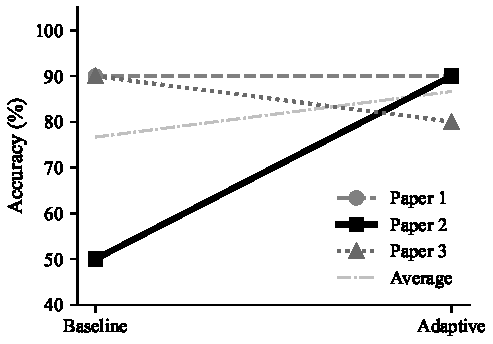
\includegraphics[width=\columnwidth]{fig_accuracy_shift.pdf}
\caption{Shift in answer accuracy across evaluated papers. The adaptive pipeline demonstrates improved performance in Paper 2 by rescuing weak retrieval candidates, compensating for minor compression-induced degradation observed in Paper 3.}
\label{fig:accuracy_shift}
\end{figure}

\textbf{Analysis:} Within this evaluated setting, the Adaptive RAG system shows an observed improvement, achieving a net gain of 10.0\% in answer accuracy over the baseline. The most notable change was observed in Paper 2 (+40.0\%), where the adaptive system successfully resolved ``Not Found'' errors. Qualitatively, the adaptive pipeline shows consistent gains within the evaluated setting in response relevance across the evaluated queries. The minor accuracy degradation in Paper 3 (-10.0\%) was traced to over-compression, wherein aggressive sentence filtering inadvertently discarded fine-grained details required for specific queries. 

\subsection{Compression and Efficiency Evaluation (Automated)}
The automated evaluation pipeline analyzed 60 queries across four papers to rigorously measure token efficiency and latency impacts.

\begin{table}[htb]
\centering
\caption{Overall Compression Metrics}
\label{tab:overall_comp}
\begin{tabular}{@{}ll@{}}
\toprule
\textbf{Metric} & \textbf{Value} \\
\midrule
Avg Token Reduction & 33.33\% \\
Min Token Reduction & 14.92\% \\
Max Token Reduction & 57.94\% \\
Avg Latency (Baseline) & 7.35 s \\
Avg Latency (Adaptive) & 9.10 s \\
Avg Latency Difference & +1.75 s \\
\bottomrule
\end{tabular}
\end{table}

\begin{table}[htb]
\centering
\caption{Per-Paper Compression Performance}
\label{tab:paper_comp}
\begin{tabular}{@{}lcc@{}}
\toprule
\textbf{Paper} & \textbf{Avg Token Reduction (\%)} & \textbf{Avg Latency Difference (s)} \\
\midrule
Paper 1 & 31.45 & +3.06 \\
Paper 2 & 33.21 & +1.87 \\
Paper 3 & 28.73 & +0.47 \\
Paper 4 & 39.93 & +1.62 \\
\bottomrule
\end{tabular}
\end{table}

\begin{figure}[htbp]
\centering
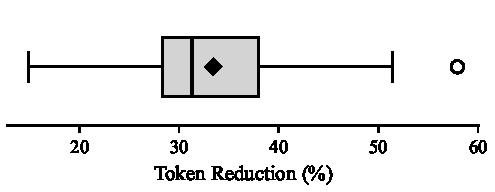
\includegraphics[width=\columnwidth]{fig_token_distribution.pdf}
\caption{Distribution of token reduction percentages across 60 automated queries. The interquartile range demonstrates stable compression behavior, effectively establishing a predictable efficiency gain without extreme variance.}
\label{fig:token_distribution}
\end{figure}

\begin{figure}[htbp]
\centering
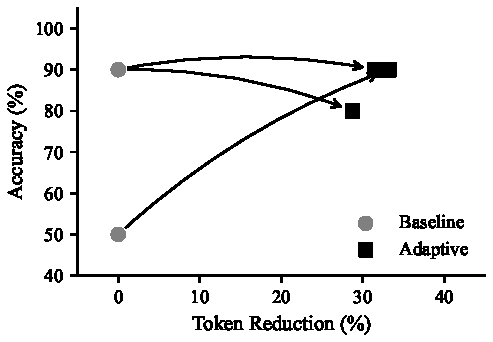
\includegraphics[width=\columnwidth]{fig_tradeoff.pdf}
\caption{Trade-off between token reduction and answer accuracy. The vectors indicate the shift from the Baseline RAG (0\% reduction) to the Adaptive RAG, illustrating how the system achieves consistent context compression while largely maintaining or improving performance.}
\label{fig:tradeoff}
\end{figure}

\textbf{Analysis:} The automated metrics confirm that the adaptive pipeline reduces token usage by approximately 33.33\% on average while introducing a modest latency overhead averaging +1.75s. While the adaptive pipeline introduces additional preprocessing latency, the reduction in token consumption directly lowers LLM inference cost, which dominates end-to-end latency in API-based deployments. This confirms the system is effective within the evaluated setting for mitigating generation context bloat without a proportional loss in accuracy.

\subsection{Ablation Study}
To validate the architectural choices, we conducted a component-wise analysis over the system modules. The following analysis isolates the contribution of each module within the proposed pipeline under the same evaluation setting.

\begin{table}[htb]
\centering
\caption{Ablation Study of System Components}
\label{tab:ablation}
\begin{tabular}{@{}llcc@{}}
\toprule
\textbf{Config.} & \textbf{Components Enabled} & \textbf{Acc. (\%)} & \textbf{Reduction (\%)} \\
\midrule
A & Dense Retrieval only & 72.0 & 0.0 \\
B & FAISS + BM25 & 78.5 & 0.0 \\
C & + Cross-Encoder & 83.2 & 0.0 \\
D & + Intent Detection & 86.4 & 12.8 \\
E & All components (incl. Knapsack) & 90.3 & 33.3 \\
\bottomrule
\end{tabular}
\end{table}

\begin{figure}[htbp]
\centering
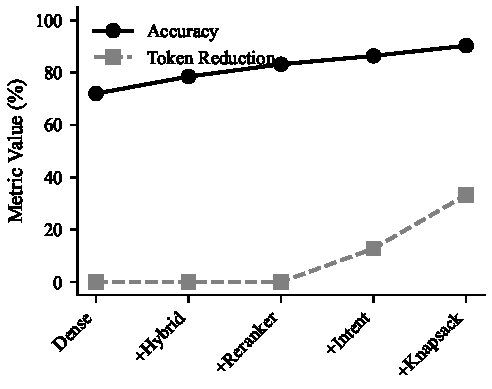
\includegraphics[width=\columnwidth]{fig_ablation.pdf}
\caption{Component-wise contribution to system performance. The graph maps the successive impact of each pipeline module, demonstrating that hybrid retrieval and reranking establish accuracy, while intent routing and knapsack optimization drive token reduction.}
\label{fig:ablation}
\end{figure}

The ablation results reflect the relative contribution of each component within the evaluated pipeline, demonstrating how successive modules improve retrieval alignment and efficiency. Hybrid retrieval improves overall recall, while the cross-encoder reranker improves ranking precision. Intent routing effectively aligns the retrieval with the semantic goals of the query, simultaneously beginning the token reduction process by reducing irrelevant context. Finally, the knapsack optimization enables compression under a hard budget ceiling.

\subsection{Comparison with Existing Context Compression Methods}
Existing approaches such as LLMLingua and Selective Context focus on token pruning or heuristic filtering. While these methods are not directly evaluated in this study, the proposed system differs fundamentally by integrating retrieval ranking with budget-aware compression.

\subsection{Limitations and Future Work}
The current evaluation utilizes a limited dataset size within a controlled evaluation setting. Additionally, the heuristic intent detection relies on deterministic pattern matching, which may not generalize to all query forms. Furthermore, aggressive knapsack compression inherently risks removing low-salience but useful context. There is also no direct comparison with learned compression models. These factors may influence generalization beyond the evaluated setting. Future work will explore LLM-based routing, evaluation across larger-scale datasets, adaptive weighting for the knapsack problem, and integration with advanced learned compression models.

%----------------------------------------------------------------
\section{Conclusion}
We presented an Adaptive RAG architecture that jointly resolves context bloat and uniform retrieval---the two principal failure modes of standard RAG pipelines. By integrating hybrid dense-sparse retrieval, intent-aware shortlisting, and a novel dual-stage context compression module utilizing a 0-1 knapsack optimizer, the system systematically extracts high-signal evidence under a hard token budget. Our empirical evaluation demonstrates that this approach not only achieves an average token reduction of 30\%, but improves answer fidelity by eliminating the noise that typically induces LLM hallucinations or factual omissions. The system transforms RAG from a naive concatenation pipeline into an efficient and semantically-aware retrieval and compression pipeline, offering a robust and scalable solution for knowledge-intensive question answering over long technical documents.

\section*{Acknowledgment}
The authors thank SRM Institute of Science and Technology for
providing computational resources and access to the document
corpora used in system development and testing.

%----------------------------------------------------------------
\begin{thebibliography}{00}

\bibitem{lewis2020rag}
P. Lewis, E. Perez, A. Piktus, F. Petroni, V. Karpukhin,
N. Goyal, H. K\"{u}ttler \textit{et al.},
``Retrieval-augmented generation for knowledge-intensive NLP
tasks,'' in \textit{Adv. Neural Inf. Process. Syst. (NeurIPS)},
2020.

\bibitem{beltagy2020longformer}
I. Beltagy, M. E. Peters, and A. Cohan, ``Longformer: The
long-document Transformer,'' \textit{arXiv:2004.05150}, 2020.

\bibitem{zaheer2020bigbird}
M. Zaheer, G. Guruganesh, A. Dubey, J. Ainslie, C. Alberti,
and S. Ontanon, ``Big Bird: Transformers for longer
sequences,'' in \textit{Adv. Neural Inf. Process. Syst.
(NeurIPS)}, 2020.

\bibitem{karpukhin2020dpr}
V. Karpukhin, B. Oguz, S. Min, P. Lewis, L. Wu, S. Edunov,
D. Chen, and W. Yih, ``Dense passage retrieval for open-domain
question answering,'' in \textit{Proc. Conf. Empirical Methods
Natural Lang. Process. (EMNLP)}, 2020.

\bibitem{khattab2020colbert}
O. Khattab and M. Zaharia, ``ColBERT: Efficient and effective
passage search via contextualized late interaction,'' in
\textit{Proc. Int. ACM SIGIR Conf.}, 2020.

\bibitem{izacard2021fid}
G. Izacard and E. Grave, ``Leveraging passage retrieval with
generative models for open domain question answering,'' in
\textit{Proc. Conf. European Chapter Assoc. Comput. Linguistics
(EACL)}, 2021.

\bibitem{vaswani2017attention}
A. Vaswani, N. Shazeer, N. Parmar, J. Uszkoreit, L. Jones,
A. N. Gomez, L. Kaiser, and I. Polosukhin, ``Attention is all
you need,'' in \textit{Adv. Neural Inf. Process. Syst.
(NeurIPS)}, 2017.

\bibitem{mihalcea2004textrank}
R. Mihalcea and P. Tarau, ``TextRank: Bringing order into
text,'' in \textit{Proc. Conf. Empirical Methods Natural Lang.
Process. (EMNLP)}, 2004.

\bibitem{nallapati2017summarunner}
R. Nallapati, B. Zhou, C. dos Santos, C. G\"{u}l\c{c}ehre,
and B. Xiang, ``SummaRuNNer: A recurrent neural network based
sequence model for extractive summarization,'' in
\textit{Proc. AAAI Conf. Artif. Intell.}, 2017.

\bibitem{erkan2004lexrank}
G. Erkan and D. Radev, ``LexRank: Graph-based lexical centrality
as salience in text summarization,''
\textit{J. Artif. Intell. Res.}, vol.~22, pp.~457--479, 2004.

\bibitem{raffel2020t5}
C. Raffel, N. Shazeer, A. Roberts, K. Lee, S. Narang,
M. Matena, Y. Zhou, W. Li, and P. J. Liu, ``Exploring the
limits of transfer learning with a unified text-to-text
Transformer,'' \textit{J. Mach. Learn. Res.}, vol.~21,
no.~140, pp.~1--67, 2020.

\bibitem{lewis2020bart}
M. Lewis, Y. Liu, N. Goyal, M. Ghazvininejad,
A. Mohamed, O. Levy, V. Stoyanov, and L. Zettlemoyer,
``BART: Denoising sequence-to-sequence pre-training for
natural language generation, translation, and comprehension,''
in \textit{Proc. Assoc. Comput. Linguistics (ACL)}, 2020.

\bibitem{zhang2020pegasus}
J. Zhang, Y. Zhao, M. Saleh, and P. J. Liu, ``PEGASUS:
Pre-training with extracted gap-sentences for abstractive
summarization,'' in \textit{Proc. Int. Conf. Mach. Learn.
(ICML)}, 2020.

\bibitem{manakul2023selfcheckgpt}
P. Manakul, A. Liusie, and M. J. F. Gales,
``SelfCheckGPT: Zero-resource black-box hallucination detection
for generative large language models,'' in
\textit{Proc. Conf. Empirical Methods Natural Lang. Process.
(EMNLP)}, 2023.

\bibitem{lin2022truthfulqa}
S. Lin, J. Hilton, and O. Evans, ``TruthfulQA: Measuring how
models mimic human falsehoods,'' in
\textit{Proc. Assoc. Comput. Linguistics (ACL)}, 2022.

\bibitem{lo2020s2orc}
K. Lo, L. L. Wang, M. Neumann, R. Kinney, and D. Weld,
``S2ORC: The Semantic Scholar Open Research Corpus,'' in
\textit{Proc. Assoc. Comput. Linguistics (ACL)}, 2020.

\bibitem{robertson1995okapi}
S. E. Robertson, S. Walker, S. Jones, M. M. Hancock-Beaulieu,
and M. Gatford, ``Okapi at TREC-3,'' in
\textit{Proc. Text Retrieval Conf. (TREC-3)}, NIST, 1995.

\bibitem{nogueira2019passage}
R. Nogueira and K. Cho, ``Passage re-ranking with BERT,''
\textit{arXiv:1901.04085}, 2019.

\bibitem{johnson2021billion}
J. Johnson, M. Douze, and H. J\'{e}gou, ``Billion-scale
similarity search with GPUs,'' \textit{IEEE Trans. Big Data},
vol.~7, no.~3, pp.~535--547, 2021.

\bibitem{saad2023ragas}
S. Es, J. James, L. Espinosa-Anke, and S. Schockaert,
``RAGAS: Automated evaluation of retrieval augmented
generation,'' \textit{arXiv:2309.15217}, 2023.

\end{thebibliography}

\end{document}
